\documentclass{article}

\usepackage[a4paper, total={6in, 8in}]{geometry}

\usepackage{amsmath}
\usepackage{amsfonts}
\usepackage{amssymb}
\usepackage[T1, T2A]{fontenc}
\usepackage[utf8]{inputenc}
\usepackage[english, russian]{babel}
\usepackage{graphics}
\usepackage{graphicx}

\geometry{
 a4paper,
 total={170mm,257mm},
 left=20mm,
 top=20mm,
 }

\author{Александр Валентинов}
\title{Лабораторная работа 3.2.4}

\begin{document}
   \subsection*{Работа 3.2.4}
   \section*{Свободные колебания в электрическом контуре}
   
   \paragraph{Цель работы:} исследование свободных колебаний в колебательном контуре.
   
   \paragraph{В работе используются:} генератор импульсов, электронное реле, магазин сопротивлений, магазин емкостей индуктивность, электронный осциллограф, LCR-измеритель.
   
   \subsubsection*{Экспериментальная установка:}
   
   \begin{figure}[h]
   \centering
   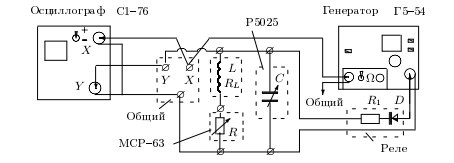
\includegraphics[width=10cm]{3_2_4.jpg} 
   \caption{Схема установки} 
   \label{fig.0} 
   \end{figure}
   
   \begin{table}[h]
   \centering 
   \caption{Параметры катушки}
   \begin{tabular}{|*{3}{c|}}
   \hline 
   $\nu, \text{Гц}$ & $L, \text{мГн}$ & $R, \text{Ом}$\\ \hline 
   50 & 145.65 & 10.516 \\ \hline 
   1.000 & 141.66 & 11.45 \\ \hline 
   5.000 & 142.36 & 136.2 \\ \hline 
   \end{tabular} 
   \end{table} 
   
   \begin{table} [h]
   \centering
   \caption{Параметры генератора}
   \begin{tabular}{|*{2}{c|}}
   \hline 
   Период импульсов $T_0$, c & 0.01 \\ \hline 
   Частота генератора $\nu$, Гц & 100 \\ \hline 
   Длительность импульсов & 5 мкс \\ \hline
   \end{tabular} 
   \end{table} 
   
   
   \subsection*{Обработка результатов}
   \subsubsection*{Вычисление периодов}
   Рассчитаем экспериментальные значения периодов колебаний по результатам измерений $x_0$, $x$, $n$. Используем формулу:
   $$ T_{\text{эксп}} = T_0\frac{x}{nx_0} $$
   Погрешность $T_{\text{эксп}}$:
   $$ \sigma_{T_{\text{эксп}}} = \sqrt{\left(\frac{T_0}{nx_0}\sigma_x\right)^2 + \left(\frac{T_0x}{nx_0^2}\sigma_{x_0}\right)^2} $$
   Найдем теоретические значения по формуле:
   \begin{equation} 
   	   \label{thperiod}
       T_{\text{теор}} = 2\pi\sqrt{LC}
   \end{equation}
   Погрешность теоретических значений пренебрежимо мала по сравнению с экспериментальными.

   Построим график $T_{\text{эксп}} = f(T_{\text{теор}})$ (рис. \ref{fig.1}). Используя метод наименьших квадратов, полагая, что график проходит через точку $(0, 0)$, найдем угловой коэффициент: 
   $$ k = 0.95 \pm 0.06 $$

   Угловой коэффициент совпадает с единицей в пределах погрешности, поэтому можно считать, что формула (\ref{thperiod}) верна.
   
   \begin{center}
   \begin{table}[h]
   \label{e1tab} 
   \centering
   \caption{Данные для эсперимента с периодами}
   \begin{tabular}{|*{7}{c|}}
   \hline 
   $x_0, \text{дел}$ & $x, \text{дел}$ & $n$ & $C, \text{мкф}$ & $T_{\text{эксп}}, \text{мc}$ & $T_{\text{теор}},\text{мс}$ & $\sigma_{T_{\text{эксп}}}, \text{мс}$\\ \hline 
   26 & 14 & 17 & 0.0200 & 0.32 & 0.339 & 0.03 \\ \hline 
   27 & 15 & 12 & 0.0400 & 0.46 & 0.480 & 0.04 \\ \hline 
   26 & 16 & 10 & 0.0800 & 0.62 & 0.678 & 0.05 \\ \hline 
   26 & 14 & 5 & 0.1500 & 1.08 & 0.929 & 0.09 \\ \hline 
   26 & 25 & 8 & 0.3000 & 1.20 & 1.310 & 0.07 \\ \hline 
   26 & 15 & 4 & 0.4000 & 1.44 & 1.520 & 0.11 \\ \hline 
   26 & 21 & 5 & 0.5000 & 1.62 & 1.700 & 0.10 \\ \hline 
   26 & 19 & 4 & 0.6000 & 1.83 & 1.860 & 0.12 \\ \hline 
   26 & 24 & 5 & 0.7000 & 1.85 & 2.010 & 0.10 \\ \hline 
   26 & 26 & 5 & 0.8000 & 2.00 & 2.140 & 0.11 \\ \hline 
   \end{tabular} 
   \end{table} 
   \end{center}
   
   \begin{figure}[h]
   \centering
   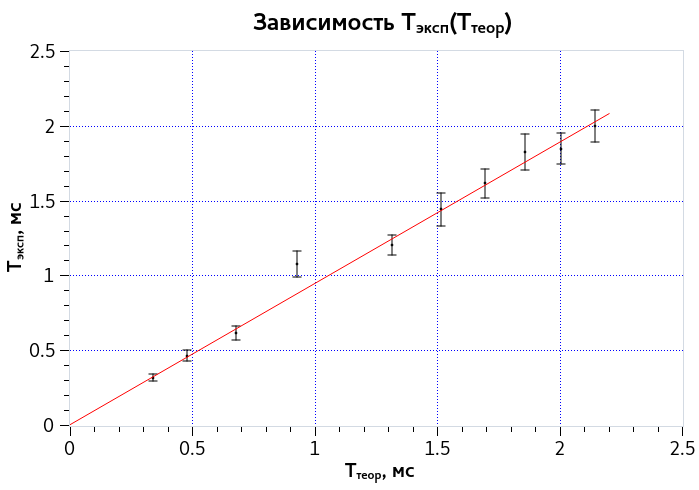
\includegraphics[width=11cm]{fig1.png} 
   \caption{График $T_{\text{эксп}}(T_{\text{теор}}) $} 
   \label{fig.1} 
   \end{figure}

   
   \subsubsection*{Критическое сопротивление, декремент затухания и добротность}
   Рассчитаем логарифмиеский декремент затухания по формуле:
   \begin{equation}
   \label{decrement}
   \Theta = \frac{1}{n} \ln\frac{U_k}{U_{k + n}} \\ 
   \end{equation}
   $$ \sigma_{\Theta} = \frac{1}{n}\sqrt{\left(\frac{\sigma_{U_{k + n}}}{U_{k + n}}\right)^2 + \left(\frac{\sigma_{U_k}}{U_k}\right)^2} $$   
   Для определения сопротивления контура сложим омическое сопротивление катушки с сопротивлением резистора:
   $$ R_{\text{конт}} = R + R_L $$
   Критическое сопротивление можно определить, используя формулу:
   $$ R_{\text{кр}} = 2\pi\sqrt{\frac{\Delta Y}{\Delta X}} $$
   $$ \sigma_{R_{\text{конт}}} = \frac{\pi}{\sqrt{\frac{\Delta Y}{\Delta X}}}\sigma_{\frac{\Delta Y}{\Delta X}} $$
   где 
   $$ X = \frac{1}{R_{кр}^2},~ Y = \frac{1}{\Theta^2} $$
   Чтобы найти $ \frac{\Delta Y}{\Delta X} $, построим график $ Y(X) $ (рис. \ref{fig.2}) и найдем его угловой коэффициент:
   $$ \frac{\Delta Y}{\Delta X} = (3.9 \pm 0.2) \text{кОм}^2 $$
   Погрешность $X$ мала по сравнению с погрешностью $Y$:
   $$ \sigma_Y = \frac{2n^2}{\ln^3\left(\frac{U_k}{U_{k+n}}\right)} \sqrt{\left(\frac{\sigma_{U_{k}}}{U_k}\right)^2 + \left(\frac{\sigma_{U_{k+n}}}{U_{k + n}}\right)^2} $$
   Получаем:
   $$ R_{\text{кр}}^{\text{граф}} = (12.4 \pm 0.3)\text{кОм} $$
   Рассчитаем теоретическое значение для критического сопротивления:
   \begin{equation}
   \label{rcritth}
   R_{\text{крит}}^{\text{теор}} = 2\sqrt{\frac{L}{C}}
   \end{equation}   
   $$ \sigma_{R_{\text{кр}}^{\text{теор}}} = 2 \frac{\sqrt{LC}}{C^2} \sigma_C $$   
   $$ R_{\text{крит}}^{\text{теор}} = (10.6 \pm 0.2) \text{кОм} $$
   Значение полученное в ходе эксперимента:
   $$ R_{\text{крит}}^{\text{эксп}} = 8 \text{кОм} $$
   Полученное значение близко к графическому результату. Результат полученный практически меньше графического и теоретического. Это может быть вызвано тем, что точность осциллографа, с помощью которого определялась апериодичность колебаний, не позволяла увидеть колебания с малой амплитудой.
   
   Рассчитаем добротность для максимального и минимального $\Theta$ по формуле:
   $$ Q = \frac{\pi}{\Theta},~~ \sigma_Q = \frac{\pi}{\Theta^2} \sigma_{\Theta} $$
   $$ Q_{\Theta_{max}}^{(1)} = 2.36 \pm 0.16 $$ 
   $$ Q_{\Theta_{min}}^{(1)} = 6.6 \pm 0.9 $$
   Рассчитаем эти же величины, используя формулу:
   \begin{equation}
   \label{qtheor}
   Q = \frac{1}{R} \sqrt{\frac{L}{C}},~~ \sigma_Q = \sqrt{\left(\frac{1}{R}\frac{\sqrt{LC}}{C^2} \sigma_C\right)^2 + \left(\frac{1}{R^2}\sqrt{\frac{L}{C}}\sigma_R\right)^2}
   \end{equation}    
   $$ Q_{\Theta_{max}}^{(2)} = 2.28 \pm 0.06 $$ 
   $$ Q_{\Theta_{min}}^{(2)} = 6.51 \pm 0.13 $$
   Полученные значения совпадают в пределах погрешности, значит теоретическая формула (\ref{qtheor}) верна.
  
   \begin{table}[h] 
   \label{e2tab}
   \centering
   \caption{Данные для эксперимента с затухающими колебаниями}
   \begin{tabular}{|*{9}{c|}}
   \hline 
   $R,~ \text{кОм}$ & $R_{\text{конт}},~ \text{кОм}$ & $ X, \text{кОм}^{-2}$ & 
   $U_k$ & $U_{k+n}$ & $n$ & $\Theta$ & $Y$ & $\sigma_Y$ \\ \hline 
   0.800 & 0.936 & 1.141 & 20 & 3 & 4 & 0.474 & 4.4 & 0.8 \\ \hline 
   1.000 & 1.136 & 0.775 & 33 & 3 & 4 & 0.599 & 2.8 & 0.3 \\ \hline 
   1.300 & 1.436 & 0.485 & 34 & 3 & 3 & 0.809 & 1.5 & 0.2 \\ \hline 
   1.500 & 1.636 & 0.374 & 35 & 3 & 3 & 0.819 & 1.5 & 0.2 \\ \hline 
   1.900 & 2.036 & 0.241 & 34 & 4 & 2 & 1.07 & 0.87 & 0.08 \\ \hline 
   2.200 & 2.336 & 0.183 & 34 & 9 & 1 & 1.33 & 0.57 & 0.04 \\ \hline 
   \end{tabular} 
   \end{table} 
   
   \begin{figure}[h]
   \centering
   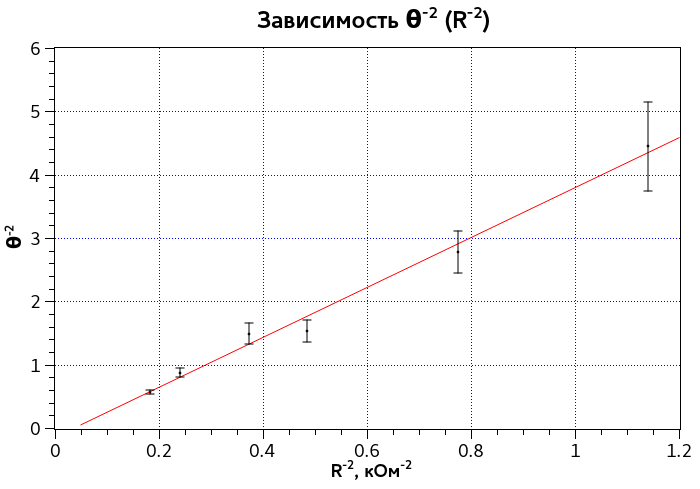
\includegraphics[width=11cm]{fig2.png} 
   \caption{Зависимость $Y(X)$} 
   \label{fig.2} 
   \end{figure}
   
   \subsubsection*{Колебания на фазовой плоскости}
   Имея спираль на плоскости $(\dot U, U)$, мы можем посчитать логарифмический декремент, пользуясь формулой (\ref{decrement}). Для этого снимем значения точек, в которых спираль пересекает ось $Y = U$: в этот момент ток равен нулю, а напряжение максимально. Количество витков спирали есть количество периодов между точками.
   $$ \Theta_{max} =  1.30 \pm 0.11 $$
   $$ \Theta_{min} = 0.46 \pm 0.04 $$
   Полученные значения совпадают с вычисленными по результатам эксперимента с графиком напряжения от времени (Таблица 2). Этот способ более точный, т.к. напряжение в момент, когда конденсатор полностью заряжен легче определить, а также осциллограф позволяет получить большее абсолютное значение напряжения с меньшей погрешностью.
   
   \begin{table}[h]
   \centering 
   \caption{Радиус спирали}
   \begin{tabular}{|*{6}{c|}}
   \hline 
   $Y$, дел, $0.1R_\text{кр}$ & 2 & 4 & 6 & 9 & 16 \\ \hline  
   \end{tabular} 
   \begin{tabular}{|*{3}{c|}}
   \hline 
   $Y$, дел, $0.3R_\text{кр}$ & 6 & 22 \\ \hline  
   \end{tabular} 
   \end{table} 
   
   
   \subsection*{Вывод}
   Эксперимент показал, что для определения периода колебаний можно пользоваться формулой (\ref{thperiod}). Для критического сопротивления справедлива формула (\ref{rcritth}). Добротность контура можно описать формулой (\ref{qtheor}).
\end{document}
